\chapter{Requirements}
\label{ch:Chapter3}
\vfill \minitoc \newpage

\section{Functional Requirements}
In this section we will delve in to the requirements needed to implement this project. %complete


\subsection{Mandatory Requirements}

The mandatory functional requirements are the following:
\begin{itemize}
    \item Editing and personalizing a postcard

	\item Sending and receiving postcards;
	
	\item Creating chat groups;
	
	\item Connecting to all friends in the service via user's stored phone number;
	
	\item Export a postcard in high quality;

    \item Build and train a Handwriting Text Recognition model.
\end{itemize}


\subsection{Optional Requirements}

\begin{itemize}
        \item Use a \gls{tts} implementation to read the postcard out loud;
        \item Using \gls{sms} based verification;
\end{itemize}

\bigskip 

\section{Overview}
\noindent

PostChat has simple and intuitive functionalities. In this chapter is shown a overview of the service, detailed explanation of every component will be provided later in this report.

\subsection{Project Architecture}
PostChat has a client made for Android using Jetpack Compose framework a server programmed in Kotlin using the Spring framework and running in the \gls{jvm}. The same server creates processes to call the \gls{ai} \gls{htr} model made in Python and uses a PostgreSQL database to store data. 

\begin{figure}[!ht]
	\centering
	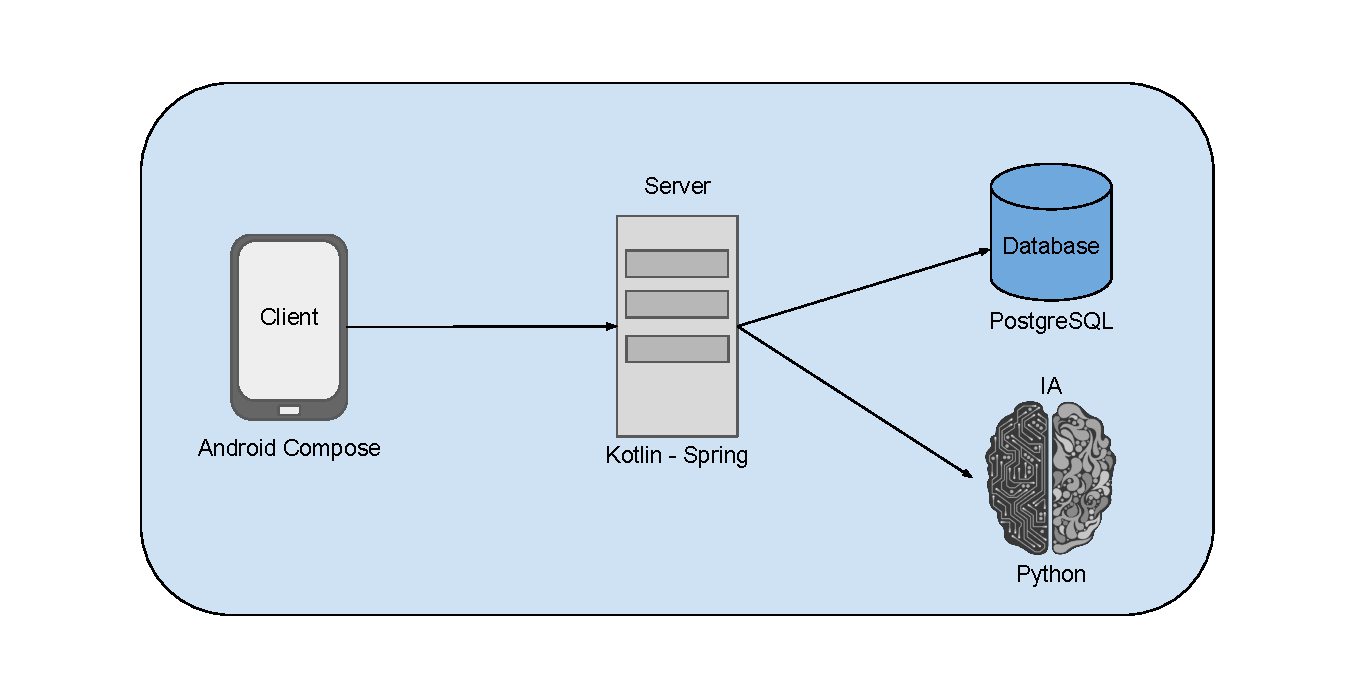
\includegraphics[width=0.9\textwidth]{./Chapter3/Figures/Project Structure}
	\caption{Project Architecture}
	\label{fig:PStruct}
\end{figure}


\subsection{Signing In}
To be able to use any of the provided functionalities its necessary for the user to sign in the service. Signing In can be either a login operation or a register operation. Its required for the user to have a valid phone number in order to perform either one of the operations.
Once registered the user will have access to all of the service functionalities.

\subsection{Connecting to Friends}
Connecting to friends in the service is simple, no need to find for a specific username simply give access to the user's phone numbers and the service will provide you with the contacts registered in it.   

\subsection{Obtaining Templates}
A template represents a potential postcard background. Every application developed to use this Web API needs to have consistency, that is, it needs to keep the templates up-to-date with the ones stored in the server.


\subsection{Creating Chat Groups}
Once registered the user can now create chats groups. These chat groups are made up of all the people the users is meant to send a postcard and/or receive from.
When sending a postcard to someone a chat group is required.  

\subsection{Sending Messages (Postcards)}
A message is referenced in this report and throughout the application development as a holder for the postcard. A message contains more information besides the postcard itself (we will delve deeper about messages in the report \ref{subsec:Message}).
Sending a postcard involves choosing a postcard template (the background of the postcard) and  writing to it. 
Internally the postcard is represented by two layers, the template and the written content, both of which are SVG's \textit{\cite{SVG}}, allowing for high quality postcards. 

\subsection{Handwriting Text Recognition}
For each message a request can be made to extract the drawn text contained in it to computer digits. To perform such operation only the drawn content is needed.

\bigskip

\paragraph{Application Flow}

The application flow can be seen in Figure~\ref{fig:AppFlow}.

\begin{figure}[!ht]
	\centering
	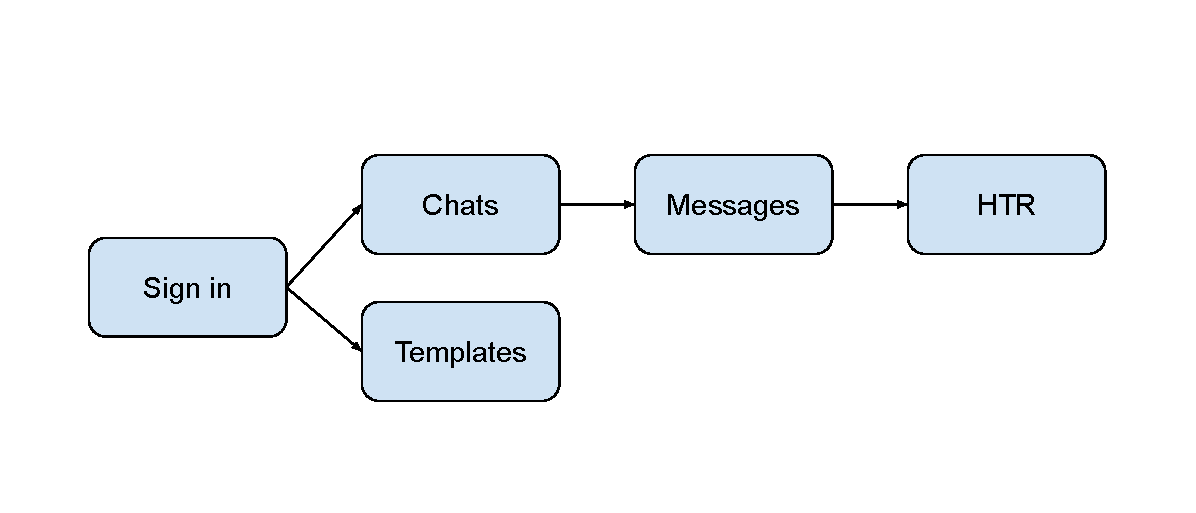
\includegraphics[width=0.75\textwidth]{./Chapter3/Figures/Application Flow}
	\caption{Application Flow}
	\label{fig:AppFlow}
\end{figure}